\documentclass[11pt]{article}

\usepackage[margin=1in]{geometry}
\usepackage{graphicx}
\usepackage{amsmath,amssymb}
\usepackage{booktabs}
\usepackage{multirow}
\usepackage{xcolor}
\usepackage[hidelinks]{hyperref}
\usepackage{url}
\usepackage[T1]{fontenc}
\usepackage{lmodern}
\usepackage{caption}
\usepackage{microtype}
\captionsetup{font=small,labelfont=bf}

\newcommand{\Zmsa}{\ensuremath{Z_{\mathrm{msa}}}}
\newcommand{\Zno}{\ensuremath{Z_{\mathrm{no}}}}
\newcommand{\eff}{eff90}

\title{What the MSA writes into an AF3-style trunk's pair representation,\\and why it helps mutation-effect prediction}

\author{Cheng Ding$^{1,\ast}$\\
\small $^{1}$School of Life Science and Technology, ShanghaiTech University, Shanghai, China\\
\small $^{\ast}$Correspondence: \texttt{dingcheng2024@shanghaitech.edu.cn}; ORCID: \href{https://orcid.org/0009-0001-7221-9066}{0009-0001-7221-9066}}

\date{}

\begin{document}
\maketitle

\begin{abstract}
Multiple sequence alignments (MSAs) have been progressively de-emphasized in
protein structure prediction: AlphaFold2 made the MSA a first-class,
recurrently processed input, whereas AlphaFold3 (AF3) and its open
implementation RosettaFold-3 (RF3) compress MSA processing into a small module
whose entire output passes once into the pair representation. Neither the AF3
nor the RF3 report measures what this channel contributes, and all existing
MSA-perturbation evidence is at the input-to-output level. Here we measure, at
the representation level, what the MSA writes into the pair representation of
an RF3 trunk, and quantify its net effect on deep mutational scanning (DMS)
prediction. Across three proteins, the MSA mildly compresses the per-mutant
pair-representation ensemble toward a family consensus (effective rank
$-16\%$ to $-42\%$; linear CKA to the no-MSA representation 0.53--0.92), yet
this compression \emph{helps} cross-position mutation-effect prediction: the
de-biased gain is $+0.14$--$0.15$ Spearman $\rho$ on the two proteins where
de-biasing was performed. A dose$\times$content decomposition attributes the
functional gain to per-column conservation ($\sim$2/3) and pairwise
covariation ($\sim$1/3), saturating at $\sim$8 MSA rows, while a generic
``shared-context tax'' compresses rank without buying function. Gating the MSA
to a single recycle installs $\sim$75\% of the geometric and $\sim$85\% of the
functional effect, and nine subsequent MSA-free recycles wash out only
$\sim$25\%: the write is one-shot and near-irreversible, a causal confirmation
of AF3's ``all information passes through the pair representation'' design.
Roughly 60\% of the MSA-specific functional advantage is reconstructible from
the no-MSA pair representation plus ESM-2 embeddings. Across proteins, the
functional gain tracks the magnitude of the representational rewrite, not raw
MSA depth: family coherence, not depth, is the operative variable.
\end{abstract}

\section{Introduction}

The multiple sequence alignment entered protein structure prediction as the
carrier of evolutionary covariation: residue pairs that co-vary across a
family are likely to be in contact, and direct-coupling methods could fold
proteins from MSAs alone, without any supervised structural data
\cite{marks2012,ahdritz2024}. AlphaFold1 converted coevolutionary statistics
from an alignment into deep-learned distance potentials \cite{senior2020};
AlphaFold2 (AF2) made the MSA a first-class
input, processed recurrently by the Evoformer alongside the pair
representation, and trained with a masked-MSA reconstruction loss
\cite{jumper2021}. AF2's own analysis documented a dose--response with a
characteristic threshold: accuracy drops substantially below $\sim$30
alignment rows and saturates beyond $\sim$100, and the authors hypothesized
that MSA information is needed early, ``to coarsely find the correct
structure,'' rather than for refinement \cite{jumper2021}.

Since then, the field has steadily de-emphasized the MSA. ESMFold removed it
outright, showing that a large protein language model (pLM) can replace MSA
processing for most targets while being up to 60$\times$ faster
\cite{lin2022}; ESM3 extended the single-sequence paradigm and its benchmarks
show the residual MSA advantage concentrated on hard targets \cite{hayes2024}.
RFdiffusion dispenses with the MSA entirely, carrying the structural prior in
pretrained weights instead \cite{watson2023}.
AlphaFold3 kept the MSA but architecturally demoted it: MSA processing is
reduced to four blocks with inexpensive pair-weighted averaging, and ``the MSA
representation is not retained and all information passes through the pair
representation'' \cite{abramson2024}. RosettaFold-3 (RF3), an open AF3-style
implementation, inherits this design \cite{corley2025}. Yet RF3's report
contains no ablation of the MSA input---its only ablation statement concerns
the MSA \emph{search tool} \cite{corley2025}---and AF3's architectural
demotion was likewise never accompanied by a measurement of what the MSA
channel contributes inside the trunk.

In parallel, a substantial literature has characterized the MSA's influence at
the input$\to$output level. Perturbing the MSA---by depth subsampling,
clustering, in-silico mutagenesis, or column masking---releases alternative
conformations from AF2 \cite{delalamo2022,waymentsteele2024,stein2022,kalakoti2025},
and removing MSA features removes learned conformational-state biases in GPCR
modeling \cite{sala2023,heo2022}. Conversely, MSA statistics remain a strong
substrate for variant-effect prediction across depths \cite{notin2023}, and
MSA-based models retain variant-effect performance that single-sequence pLMs
lose as they scale \cite{akiyama2025}. What is missing is a representation-level
account: no study has quantified what the MSA writes \emph{into the pair
representation itself}---in terms of rank, representational similarity, or
preservation of mutation-conditioned directions---nor decomposed the write
into its information channels, nor tested causally whether the write is
reversible, nor measured its net functional effect on mutation-effect
prediction with depth-matched controls inside one fixed trunk.

We perform these measurements in RF3, using its pair representation
($Z_{\mathrm{II}}$, captured at the distogram head) as the readout, on three
proteins with DMS data spanning shallow to deep MSAs (15 to 512 rows). We ask
four questions. (i) Geometrically, what does the MSA do to the ensemble of
per-mutant pair representations? (ii) Functionally, does the write help or
hurt cross-position mutation-effect prediction, and by how much after
correcting for selection and preprocessing biases? (iii) What is the write
made of---shared context, per-column conservation, or pairwise
covariation---and when in the trunk's recycles is it installed? (iv) How much
of the written content is already available from the no-MSA pair
representation and from ESM-2 embeddings? We find that the MSA performs a
one-shot, near-irreversible family-consensus write; that this write is
functionally \emph{beneficial} for DMS prediction; that conservation carries
most of the benefit; and that the benefit scales with the magnitude of the
rewrite rather than with alignment depth. We also report two methodological
artifacts we encountered---a feature-slicing bug that initially inverted our
headline conclusion, and a standardization-convention inconsistency---because
both are silent, severe, and likely to affect similar analyses.

\section{Results}

\subsection{The MSA mildly compresses the pair representation, and this helps prediction}
\label{sec:threeprotein}

We extracted the pair representation of RF3 for every single-point mutant of
three proteins, with and without the MSA, slicing each mutant's representation
at the true mutation site (row and column; Methods). The three proteins span
three MSA regimes: the SARS-CoV-2 spike receptor-binding domain (RBD; 15-row
shallow MSA, $N{=}3998$ mutants), human caspase-3 (CASP3; 69 Swiss-Prot
homolog rows, homodimer), and the $\lambda$ repressor CI domain (CI; 512-row
deep UniRef30 MSA).

On all three proteins, the MSA compresses the per-mutant representation
ensemble toward a family consensus, but mildly (Fig.~\ref{fig:geometry},
Table~\ref{tab:threeprotein}): the effective rank at 90\% variance drops by
16--42\% (RBD $231{\to}171$; CASP3 $333{\to}193$; CI $61{\to}51$), the
with/without-MSA representations remain substantially aligned (linear CKA
0.527/0.553/0.917), and per-mutant delta directions (mutant minus wild type)
are partially preserved (median cosine 0.474/0.362/0.844) while delta norms
are amplified rather than suppressed (RBD ratio 1.21). This is a partial
subspace compression with substantial representational continuity---not an
erasure of mutation-conditioned structure.

Supervised probing against DMS labels shows that this compression is
functionally beneficial (Fig.~\ref{fig:singlemod}). Under the canonical
split-paired protocol (Methods), the MSA-side representation outperforms the
no-MSA side on all three proteins: RBD $+0.179$ and $+0.204$ Spearman $\rho$
in two independent full-set runs (5/5 position splits positive in each; the
0.025 run-to-run spread matches our measured cross-process noise floor), CASP3
$+0.162$ (5/5), and CI $+0.075$ (4/5). The naive expectation that compressing
per-mutant distinctions should destroy mutation information is wrong: the
family-consensus write \emph{re-encodes} mutation signals toward family
evolutionary statistics, which is precisely the signal that must generalize
across positions.

\begin{table}[t]
\centering
\caption{\textbf{The MSA pins the pair representation mildly and improves
cross-position mutation-effect prediction on three proteins.} \eff{} =
effective rank at 90\% variance of the centered per-mutant feature ensemble;
CKA = linear CKA between with-MSA and no-MSA representations; dCos = median
cosine of per-mutant delta directions (MSA vs.\ no-MSA); $\Delta\rho$ =
split-paired supervised gain (sp$_{\mathrm{msa}}{-}$sp$_{\mathrm{no}}$),
best-epoch validation under overall standardization (optimistic; see
\S\ref{sec:honest}); honest = de-biased estimate (\S\ref{sec:honest}). Splits
= position splits with positive gain out of five.}
\label{tab:threeprotein}
\small
\begin{tabular}{llccccc}
\toprule
Protein & MSA rows & \eff{} no$\to$MSA & CKA & dCos & $\Delta\rho$ (best-val) & Honest $\Delta\rho$ \\
\midrule
RBD   & 15  & $231\to171$ ($-26\%$) & 0.527 & 0.474 & $+0.179$/$+0.204$ (5/5, 2 runs) & $+0.14$--$0.15$ \\
CASP3 & 69  & $333\to193$ ($-42\%$) & 0.553 & 0.362 & $+0.162$ (5/5) & $+0.14$--$0.18$ \\
CI    & 512 & $61\to51$ ($-16\%$)   & 0.917 & 0.844 & $+0.075$ (4/5) & --- \\
\bottomrule
\end{tabular}
\end{table}

\subsection{An honest effect size: de-biasing selection and preprocessing}
\label{sec:honest}

The gains above are best-epoch validation scores under a standardization that
pools all samples before splitting, and are optimistically biased by two
independent routes. First, selecting the best epoch on a single validation set
overfits it: in a dual-validation design (60/20/20 cross-position split), the
selection optimism is $+0.04$ to $+0.09$ depending on the cell, worst for the
MSA-only probe ($+0.094$, 5/5 splits). Second, fitting per-position
standardization statistics on all samples leaks validation/test statistics
into the transform; re-fitting them on training rows only (``strict'') lowers
the MSA-only probe from 0.644 to 0.589 on RBD ($-0.055$, 15/15 paired runs)
while the no-MSA probe drops only 0.022.

Two independent de-biasing corrections converge on the same number. On RBD,
held-out-test evaluation gives $+0.141$ (test at the val-selected epoch) and
$+0.143$ (best test); strict train-only standardization gives $+0.146$. On
CASP3, the dual-validation replication gives honest gains of $+0.142$ to
$+0.183$ depending on estimator. We therefore report the \textbf{honest RBD
MSA effect as $+0.14$--$0.15$ Spearman $\rho$} (honest absolute probe level
$\rho \approx 0.59$), with the CASP3 effect in the same magnitude class
($+0.14$--$0.18$); the best-validation figures of \S\ref{sec:threeprotein}
should be read as optimistic upper bounds. The RBD val-set asymmetry that
drives part of the selection optimism is protein-specific: a pre-registered
replication on CASP3 falsified the hypothesis that stronger geometric pinning
causes it (CASP3 pins harder, $-42\%$ vs.\ $-26\%$, yet shows no such offset),
and which single stream is stable versus noisy inverts between the two
proteins. Throughout, we treat effects within $\pm 0.02$ as
uninterpretable---this is the measured cross-process noise floor of the
pipeline (Methods).

\subsection{Content decomposition: a shared-context tax, conservation, and covariation}
\label{sec:e1}

What in the MSA produces these effects? We constructed eight RBD MSA arms that
orthogonalize dose and content: four real-alignment depths (1, 4, 8, and all
15 rows), a consensus arm (every row replaced by the consensus sequence,
destroying variation but keeping the profile), a column-shuffle arm
(per-column amino-acid frequencies preserved, covariation destroyed), a
row-shuffle arm, and a random-sequence arm (Fig.~\ref{fig:arms},
Table~\ref{tab:e1}). Supervised numbers in this subsection come from the
E1 dose-curve protocol (500-mutant subset, scalar standardization; Methods);
arm comparisons are within-protocol.

Three channels separate cleanly. First, a \textbf{shared-context tax}: any
alignment-like input---including random sequences---compresses the
representation (effective rank 181 for no-MSA down to $\sim$149--155 for
random/row-shuffled contexts). Presenting any shared per-residue context
diverts representational capacity, but this buys \emph{no} function: the
honest zero-content baseline is the 1-row alignment (depth01, $\rho=0.490$),
not the no-MSA input ($0.414$)---the $+0.076$ gap between them is a
featurization-path effect of presenting an alignment at all---and random or
row-shuffled contexts sit at or below depth01 ($0.479$, $0.477$). Second,
\textbf{per-column conservation} carries about two-thirds of the biological
gain: column-shuffled profiles (frequencies without covariation) reach
$+0.106$ over depth01, of which the profile itself (consensus) contributes
almost nothing ($+0.011$); the conservation-specific step from consensus to
column-shuffled frequencies is $+0.095$. Consistent with this, the consensus
and column-shuffle arms are nearly indistinguishable in rank ($156$ vs.\
$150$) but separate sharply in how they preserve mutation directions (dCos
$0.815$ vs.\ $0.548$). Third, \textbf{pairwise covariation} contributes the
remaining third: restoring true rows (full15) adds $+0.042$ over
column-shuffle. The dose response saturates early---depth04 $+0.046$, depth08
$+0.136$, full15 $+0.148$ over depth01, with effective rank plateauing from
$\sim$8 rows---so the functional gain is monotone in conservation/covariation
\emph{content}, not in sequence count.

\begin{table}[t]
\centering
\caption{\textbf{E1 dose$\times$content arms (RBD, 500-mutant subset
protocol).} \eff{} = effective rank at 90\% variance; $\rho$ = supervised
cross-position Spearman (500-subset protocol, not comparable to the canonical
full-set protocol); gain = $\rho$ minus the depth01 baseline. The no-MSA
input is \emph{not} the honest baseline (see text).}
\label{tab:e1}
\small
\begin{tabular}{llccc}
\toprule
Arm & Content & \eff{} & $\rho$ & gain vs depth01 \\
\midrule
noMSA      & none (sequence only)          & 181 & 0.414 & $-0.076$ \\
depth01    & single row (baseline)         & 165 & 0.490 & --- \\
random     & shared context, no biology    & 149 & 0.479 & $-0.011$ \\
rowshuffle & shared context, no biology    & 155 & 0.477 & $-0.013$ \\
consensus  & profile only                  & 156 & 0.501 & $+0.011$ \\
colshuffle & $+$ per-column frequencies    & 150 & 0.596 & $+0.106$ \\
depth04    & 4 real rows                   & 157 & 0.536 & $+0.046$ \\
depth08    & 8 real rows                   & 138 & 0.626 & $+0.136$ \\
full15     & all 15 rows (with covariation)& 139 & 0.638 & $+0.148$ \\
\bottomrule
\end{tabular}
\end{table}

\subsection{The write happens once and is near-irreversible}
\label{sec:e7}

In RF3, as in AF3, the MSA enters the pair representation through
outer-product-mean modules in the first four MSA blocks of each recycle; the
pair representation is the only carrier thereafter. We tested the temporal
structure of this write by gating MSA exposure to the first $K$ of the
network's ten recycles (Table~\ref{tab:e7}). A single MSA recycle ($K{=}1$)
installs $\sim$75\% of the total effective-rank drop (181$\to$150 of the
181$\to$139 full effect) and $\sim$85\% of the total functional gain
($\rho=0.605$ of the way from 0.414 to 0.638); $K{=}2$ and $K{=}3$ saturate
the remainder. Nine subsequent MSA-free recycles wash out only $\sim$25\% of
the geometric effect: the trunk cannot self-correct the family-consensus write
once installed. The near-equality of the $K{=}1$ and column-shuffle arms in
effective rank (150 both) triangulates the mechanism: a single exposure
already deposits the profile-plus-one-shot-covariation content, and repeated
injection only deepens it marginally. This is a causal, representation-level
confirmation of AF3's architectural statement that the MSA representation is
not retained and all information passes through the pair representation
\cite{abramson2024}---and it sharpens AF2's dose--response observation
\cite{jumper2021}: not only is $\sim$8--15 rows enough, a single pass of
processing is enough.

\begin{table}[t]
\centering
\caption{\textbf{Write-once dynamics (E7, RBD).} MSA exposure gated to the
first $K$ recycles. Geometric share = fraction of the full \eff{} drop
($181{\to}139$); functional share = fraction of the full $\rho$ gain
($0.414{\to}0.638$).}
\label{tab:e7}
\small
\begin{tabular}{lcccc}
\toprule
Arm & \eff{} & $\rho$ (500-subset) & geometric share & functional share \\
\midrule
noMSA          & 181 & 0.414 & 0\% & 0\% \\
$K{=}1$        & 150 & 0.605 & 74\% & 85\% \\
$K{=}2$        & 145 & 0.628 & 86\% & 96\% \\
$K{=}3$        & 144 & 0.609 & 88\% & 87\% \\
full15 (10 rc) & 139 & 0.638 & 100\% & 100\% \\
\bottomrule
\end{tabular}
\end{table}

\subsection{The MSA stream subsumes the no-MSA structural signal and duplicates ESM-2}
\label{sec:triad}

We next asked how the MSA-written pair representation relates to the two other
mutation-prediction signals available to the trunk setting: the no-MSA pair
representation \Zno{} (structure without family context) and per-mutant ESM-2
650M embeddings (FAESM; evolution without structure). Using a validated
fusion architecture with dead-stream controls (zeros streams; Methods), we
computed each signal's marginal contribution over the others on all three
proteins (Fig.~\ref{fig:triad}, Table~\ref{tab:triad}).

On RBD, \Zmsa{} alone ($\rho=0.644$) dominates: adding FAESM on top of \Zmsa{}
changes performance by $-0.005$, and adding \Zno{} on top of
$(\Zmsa{+}\mathrm{FAESM})$ by $+0.002$---both inside the $\pm0.02$ noise
floor---while FAESM does carry $+0.075$ over a \Zno{} backbone. The MSA write
thus subsumes the no-MSA structural signal and duplicates the ESM signal
simultaneously on this protein. Cross-protein, the no-MSA marginal stays
$\approx 0$ everywhere ($-0.001$ CASP3, $+0.008$ CI), but the ESM duplication
is protein-dependent: on CASP3, FAESM adds $+0.051$ over \Zmsa{} (5/5
splits), so the MSA does not fully subsume ESM there; on CI the marginal
($-0.039$) is unresolved, driven by one outlier split at small $N$. Under
strict train-only standardization, every fusion cell drops by 0.007--0.039 but
all marginal conclusions are unchanged; only the absolute levels and the
\Zmsa{}-over-\Zno{} magnitude are convention-dependent.

\begin{table}[t]
\centering
\caption{\textbf{Fusion triad, three proteins (best-validation, overall
standardization).} Single-stream probes (sp) and dead-stream-corrected
marginals of FAESM over \Zmsa{} and of \Zno{} over $(\Zmsa{+}\mathrm{FAESM})$.
The CI FAESM marginal is driven by one outlier split (2/5 positive) and should
be read as unresolved.}
\label{tab:triad}
\small
\begin{tabular}{lccccc}
\toprule
Protein & sp$_{\mathrm{no}}$ & sp$_{\mathrm{msa}}$ & sp$_{\mathrm{faesm}}$ &
FAESM $\mid$ \Zmsa{} & \Zno{} $\mid$ (\Zmsa{}+FAESM) \\
\midrule
RBD   & 0.465 & 0.644 & 0.484 & $-0.005$ & $+0.002$ \\
CASP3 & 0.394 & 0.556 & 0.584 & $+0.051$ (5/5) & $-0.001$ \\
CI    & 0.374 & 0.449 & 0.452 & $-0.039$ (noisy) & $+0.008$ \\
\bottomrule
\end{tabular}
\end{table}

The information accounting, however, is \emph{opposite} to the optimization
accounting. Late in training, the ESM encoder's gradient dominates on all
three proteins (RBD gradient-norm ratios $f/z\approx6.5$, $f/m\approx2.7$;
CASP3 and CI $f/m\approx3.5$--$3.8$), even where its information marginal is
zero. We tested causally whether this gradient dominance suppresses the MSA
stream's contribution on RBD with two interventions that rebalance gradients
without adding information. Adding Gaussian noise to the ESM stream produces
an inverted-U: validation $\rho$ rises from 0.649 to a peak of 0.662 at 75\%
noise (paired $+0.013$) and returns to baseline at 100\% noise (0.648, equal
to the dead-stream control 0.655 within noise), while the late $f/z$ gradient
ratio collapses monotonically from 2.91 to 0.04. Slowing the ESM encoder's
learning rate (content-cost-free) gives a plateau with the cleanest single arm
at $\lambda=0.25$ ($+0.014$, 5/5 splits). Both interventions recover the same
small slice ($+0.013$--$0.014$) of the MSA stream's contribution. The reading
is that on RBD the ESM stream is information-redundant with the MSA write yet
optimization-harmful to it---gradient dominance is not information dominance.

\subsection{The MSA write is partially reconstructible from no-MSA structure and ESM-2}
\label{sec:d1}

If the MSA write is a family-consensus re-encoding, how much of it is already
implicit in other features? We trained regressors from $(\Zno{}, \mathrm{FAESM})$
to \Zmsa{} across an architecture ladder (linear, MLP-256/512, 1--2-layer
transformers; Fig.~\ref{fig:d1}). Validation CKA against the real \Zmsa{}
rises from 0.74 (linear) to a plateau of $\sim$0.80--0.83 from MLP-512
(transformers do not exceed the MLP under best-epoch selection), with
validation $R^2$ still climbing slowly (0.25$\to$0.36). Functionally, a
transformer-reconstructed \Zmsa{} recovers $\sim$60\% of the real MSA stream's
prediction advantage over \Zno{} ($\rho$: \Zno{} 0.446, reconstructed 0.575,
real 0.663), matching the geometric fidelity. The remaining $\sim$40\% is
MSA-specific content that is not a learnable function of the other two
modalities at these scales.

Three controls sharpen the interpretation (Fig.~\ref{fig:xattn}). First, a
depth ladder (2--8 transformer layers) with train--validation CKA gaps shows
the high reconstruction fidelity is mostly generalization, not memorization
(gap $+0.09$ at depth 8). Second, an orthogonal one-hot encoding of amino-acid
identity---carrying only sequence, no evolution---reconstructs far worse at
every depth (CKA $\sim$0.5, non-monotonic, with a train--validation gap that
\emph{grows} with depth), so the reconstructible content is genuine
evolutionary information, not trivial sequence-to-structure memorization.
Third, a naive concatenation architecture masks \Zno{}'s contribution (the
128-dim \Zno{} is swamped by the 1280-dim ESM stream); with separate
per-modality encoders and CKA as the training objective, the hierarchy
stabilizes across depth at both-streams 0.81 $>$ ESM-only 0.75--0.76 $>$
\Zno{}-only 0.72. The information hierarchy for reconstructing the MSA write
is therefore: ESM (evolution) strongest, no-MSA pair structure a real but
smaller contributor, pure sequence identity far behind---consistent with the
ESMFold-era observation that language models absorb MSA-like information
\cite{lin2022}, now measured at the representation level.

\subsection{The functional gain tracks the magnitude of the rewrite, not MSA depth}
\label{sec:law}

Across the three proteins, the supervised gain is ordered by how hard the MSA
rewrites the representation, not by how deep the alignment is: RBD's shallow,
coherent 15-row MSA produces the hardest consensus (lowest CKA 0.527) and the
largest gain; CASP3's 69-row MSA compresses rank the most ($-42\%$) with an
intermediate gain; CI's deep-but-diverse 512-row MSA produces the softest
consensus (CKA 0.917) and the smallest gain ($+0.075$). Within RBD, the arm
series shows the same coupling: conservation-bearing arms rewrite mutation
directions more (lower dCos) and predict better. Family \emph{coherence}, not
raw depth, is the operative variable---a refinement of the naive
``deeper alignment = more information'' assumption and a complement to AF2's
$\sim$30-sequence threshold, which concerns family identification
\cite{jumper2021}.

\section{Discussion}

\subsection{Relation to prior work}

Our results sit between two literatures that have largely talked past each
other. The MSA-perturbation family showed, at the structure-output level, that
the default MSA pins predictors toward single, family-consensus
conformations---subsampling, clustering, or masking the MSA releases
alternative states \cite{delalamo2022,waymentsteele2024,stein2022,kalakoti2025},
and removing MSA features removes training-set state biases
\cite{heo2022,sala2023,saldano2022}; fold-switcher studies find the default
pipeline captures one of two conformers, sometimes via outright memorization
that bypasses the coevolution channel \cite{chakravarty2022,chakravarty2024}. The variant-effect literature showed the
opposite valence: MSA statistics are a consistently useful substrate across
depths \cite{notin2023}, and MSA-based models retain variant-effect
performance that scaling single-sequence models sacrifices
\cite{akiyama2025,notin2022}. Our representation-level measurements reconcile
the two: the \emph{same} family-consensus write that compresses the pair
representation toward family statistics is the write that supplies the
evolutionary signal DMS prediction needs. The compression and the benefit are
not in tension; they are the same operation viewed geometrically and
functionally.

For AF3-style trunks specifically, the write-once result
(\S\ref{sec:e7}) converts an architectural statement---the MSA representation
is not retained \cite{abramson2024}---into a measured causal property: the
write is installed in the first recycle and cannot be undone by the remaining
recycles. The early saturation ($\sim$8 rows; \S\ref{sec:e1}) is shallower
than AF2's $\sim$30-row threshold \cite{jumper2021}, though the comparison is
between different objects (representation-level function in a frozen trunk
vs.\ end-to-end structure accuracy). The partial reconstructibility of the
write from ESM-2 embeddings (\S\ref{sec:d1}) gives a representation-level
footing to ESMFold's inference that language models learn MSA-like information
\cite{lin2022}, and to ESM3's benchmark finding that the residual MSA
advantage concentrates on hard targets \cite{hayes2024}: here, even a
15-row MSA writes content that is only $\sim$60\% recoverable from a 650M
language model plus the no-MSA structure (mirroring at the representation level
the output-level observation that the covariation channel is often dispensable
even for complexes \cite{mirdita2022}). Practically, for DMS prediction with
AF3-style features, an MSA---even a shallow one---is worth its cost; and where
a pLM stream is fused with the MSA-bearing stream, its optimization dominance
should be managed (noise or learning-rate pacing), since information
redundancy does not imply optimization neutrality.

\subsection{Methodological cautions: two silent artifacts}
\label{sec:caution}

Two artifacts we encountered deserve emphasis because they are silent and
likely general. First, \emph{feature slicing}: an early version of our
extraction saved the pair-representation row at position 0 for every mutant
instead of the row at the mutation site. Because position 0 barely varies
across mutants, the with-MSA ensemble looked artificially low-rank (effective
rank 30 rather than 171) and the supervised signal looked destroyed ($-40\%$
rather than $+0.14$--$0.15$)---the contrast against the correctly sliced
no-MSA features was entirely bogus. Any per-mutant structural feature pipeline
should verify, explicitly, that the slice index tracks the mutation site; we
now treat this as a mandatory sanity check. Second, \emph{standardization
conventions and evaluation hygiene}: three per-residue standardization
conventions coexisted in our pipeline, and the scalar-per-position variant
specifically degraded fusion cells ($+0.037$ spurious difference on one cell)
while leaving single-modality probes robust; separately, fitting
standardization statistics before splitting inflated the MSA-side probe by up
to $+0.055$, and single-validation best-epoch selection added a further
$+0.04$--$0.09$. None of these biases changed any qualitative conclusion---the
triad ordering and all headline directions are convention-robust---but each is
large enough to manufacture or destroy a publishable effect at the margins,
and each was invisible until probed adversarially. We report de-biased numbers
as primary (\S\ref{sec:honest}) and archive both conventions.

\subsection{Limitations}

Several boundaries qualify the claims. (i) A single trunk: all measurements
are in RF3; although RF3 implements the AF3 architecture \cite{corley2025},
trained-weight specifics may matter, and AF2-style trunks with a retained MSA
track may behave differently. (ii) Three proteins, one label each, all
single-point substitutions; the CI estimate rests on only 351 mutants and one
of its marginals is unresolved. (iii) The de-biasing protocols were applied to
RBD and CASP3; the CI gain ($+0.075$, 4/5) is a best-validation figure and may
shrink similarly. (iv) The E1 decomposition was run on the RBD's shallow
15-row MSA; whether the conservation/covariation ratio holds for deep
alignments is untested. (v) The functional readout is a small supervised head
on frozen features; fine-tuning regimes could redistribute the benefit.
(vi) The gradient-rebalancing gains (\S\ref{sec:triad}) are small
($+0.013$--$0.014$) and demonstrated on RBD only; the noise-interior arm is
statistically soft (3/5 splits), with the learning-rate arm the cleaner
evidence (5/5).

\section{Methods}

\subsection{Proteins, DMS data, and MSAs}

Three proteins with deep mutational scanning data were used. RBD: the
SARS-CoV-2 spike receptor-binding domain (201-aa construct), ACE2-binding
labels (bind\_avg) from the yeast-display scan of Starr et al.\ \cite{starr2020},
$N{=}3998$ single-point mutants. CASP3: human caspase-3 (homodimer, 244
positions per chain, 488 tokens), fluorescence activity labels from the
microfluidic scan of Roychowdhury and Romero \cite{roychowdhury2022}, 1469
single-point mutants. CI: the $\lambda$ repressor CI domain (237-aa construct,
59 assayed positions), DMS\_score labels from ProteinGym \cite{notin2023},
$N{=}351$ mutants. MSAs: RBD uses a pre-existing curated alignment with 15
full-length rows; CASP3 uses 69 Swiss-Prot homolog rows and CI 512 UniRef30
rows, both built locally with MMseqs2.

\subsection{Feature extraction}

Pair representations were extracted from RF3 \cite{corley2025} by saving the
pair tensor $Z_{\mathrm{II}}$ ($L{\times}L{\times}128$) after the distogram
head through an environment-gated hook in the model's forward pass, once per
mutant, with and without the MSA. Per-mutant features are the row and column
at the true mutation site, stacked ($2{\times}L{\times}128$); the slicing
index was verified against known mutation positions after discovery of the
position-0 slicing artifact (\S\ref{sec:caution}). ESM-2 650M
(\texttt{esm2\_t33\_650M\_UR50D}) final-layer per-residue embeddings
\cite{lin2022} were computed per mutant (FAESM, $L{\times}1280$).

\subsection{Geometric metrics}

Let $X \in \mathbb{R}^{N\times d}$ be the centered matrix of per-mutant
flattened site features. Effective rank at 90\% variance (\eff{}) is the
number of principal components needed to explain 90\% of total variance.
Representational similarity between with-MSA and no-MSA ensembles is linear
CKA \cite{kornblith2019}. Mutation-direction preservation (dCos) is the median
cosine similarity, over mutants, between the with-MSA and no-MSA delta vectors
(mutant minus wild type); norm suppression/amplification is the median ratio
of delta norms.

\subsection{Supervised probing}

Two protocols are used and are not numerically interchangeable. The
\emph{canonical} protocol (three-protein geometry/function runs, fusion
matrices, distillation): a small transformer head (SinglePredictorV2) on
frozen features; per-position, per-channel z-scoring; cross-position 70/30
splits (5 seeds) with 3 head initializations (15 paired runs per cell); 300
epochs, AdamW (lr $10^{-4}$, weight decay 0.05), cosine schedule, MSE loss,
best-epoch validation Spearman $\rho$. Fusion cells use a cross-attention
fusion block with an orthogonality penalty and dead-stream (zeros) controls on
identical split$\times$init grids. The \emph{E1/E7 dose-curve} protocol:
a lighter per-position head, per-position scalar standardization, and a
500-mutant stride-8 subset of RBD; arm comparisons are made only within this
protocol (control experiments place the convention effect on single-modality
cells within $\pm0.02$). Recycle gating (E7) uses an environment variable that
zeroes the MSA input after the first $K$ recycles.

\subsection{De-biasing and statistics}

\emph{Strict standardization} fits per-position, per-channel statistics on
training rows only and freezes them onto validation/test. The
\emph{dual-validation} protocol uses 60/20/20 cross-position splits with the
second validation fold as a held-out test. All reported effects are
split-paired (paired across split$\times$initialization replicates). Effects
within $\pm0.02$ Spearman $\rho$ are treated as uninterpretable: this is the
measured cross-process/cross-GPU noise floor of the pipeline. We use
``consistent'' only when the sign is shared by at least 3 of 5 (typically 5 of
5) paired splits.

\subsection{Distillation (D1)}

Regressors from $(\Zno{}, \mathrm{FAESM})$ to \Zmsa{} were trained under
per-channel standardization (3 splits $\times$ 2 initializations, best-epoch
validation): linear, MLP with 256/512 hidden units, and 1--8-layer
transformers, in both naive-concatenation and separate-encoder (cross-attention)
variants, the latter trained with a CKA objective; controls replaced one input
modality or substituted a fixed orthogonal one-hot amino-acid codebook.
Functional equivalence of reconstructed \Zmsa{} was measured by training the
standard head on reconstructed features.

\section*{Data availability}

All analysis scripts, archived result files, and the claim-level provenance
ledger accompanying this manuscript are publicly available at
\url{https://github.com/Lizon1c/rf3-msa-pair-representation}; embeddings will
be deposited on request / upon publication.

\begin{thebibliography}{99}

\bibitem{jumper2021}
Jumper J, et al.
\newblock Highly accurate protein structure prediction with AlphaFold.
\newblock \emph{Nature} 596:583--589, 2021.
\newblock doi:10.1038/s41586-021-03819-2.

\bibitem{abramson2024}
Abramson J, et al.
\newblock Accurate structure prediction of biomolecular interactions with
AlphaFold 3.
\newblock \emph{Nature} 630:493--500, 2024.
\newblock doi:10.1038/s41586-024-07487-w.

\bibitem{lin2022}
Lin Z, et al.
\newblock Evolutionary-scale prediction of atomic-level protein structure with
a language model.
\newblock \emph{Science} 379:1123--1130, 2023.
\newblock doi:10.1101/2022.07.20.500902.

\bibitem{hayes2024}
Hayes T, et al.
\newblock Simulating 500 million years of evolution with a language model.
\newblock \emph{Science} 385:eado9336, 2025.
\newblock doi:10.1101/2024.07.01.600583.

\bibitem{corley2025}
Corley M, et al.
\newblock AtomWorks and RosettaFold-3.
\newblock \emph{bioRxiv} 2025.08.14.670328, 2025.

\bibitem{watson2023}
Watson JL, et al.
\newblock De novo design of protein structure and function with RFdiffusion.
\newblock \emph{Nature} 620:1075--1084, 2023.
\newblock doi:10.1038/s41586-023-06415-8.

\bibitem{senior2020}
Senior AW, et al.
\newblock Improved protein structure prediction using potentials from deep
learning.
\newblock \emph{Nature} 577:706--710, 2020.
\newblock doi:10.1038/s41586-019-1923-7.

\bibitem{marks2012}
Marks DS, Hopf TA, Sander C.
\newblock Protein structure prediction from sequence variation.
\newblock \emph{Nature Structural \& Molecular Biology} 19:1293--1301, 2012.

\bibitem{delalamo2022}
del Alamo D, Sala D, Mchaourab HS, Meiler J.
\newblock Sampling alternative conformational states of transporters and
receptors with AlphaFold2.
\newblock \emph{eLife} 11:e75751, 2022.

\bibitem{stein2022}
Stein RA, Mchaourab HS.
\newblock SPEACH\_AF: Sampling protein ensembles and conformational
heterogeneity with AlphaFold2.
\newblock \emph{PLoS Computational Biology} 18(8):e1010483, 2022.

\bibitem{waymentsteele2024}
Wayment-Steele HK, et al.
\newblock Predicting multiple conformations via sequence clustering and
AlphaFold2.
\newblock \emph{Nature} 625:832--839, 2024.

\bibitem{kalakoti2025}
Kalakoti Y, Wallner B.
\newblock AFsample2 predicts multiple conformations and ensembles with
AlphaFold2.
\newblock \emph{Communications Biology} 8:373, 2025.

\bibitem{saldano2022}
Salda{\~n}o TE, et al.
\newblock Impact of protein conformational diversity on AlphaFold predictions.
\newblock \emph{Bioinformatics} 38(10):2742--2748, 2022.

\bibitem{sala2023}
Sala D, Hildebrand PW, Meiler J.
\newblock Biasing AlphaFold2 to predict GPCRs and kinases with user-defined
functional or structural properties.
\newblock \emph{Frontiers in Molecular Biosciences} 10:1121962, 2023.

\bibitem{heo2022}
Heo L, Feig M.
\newblock Multi-state modeling of G-protein coupled receptors at experimental
accuracy.
\newblock \emph{Proteins} 90(11):1873--1885, 2022.

\bibitem{mirdita2022}
Mirdita M, et al.
\newblock ColabFold: making protein folding accessible to all.
\newblock \emph{Nature Methods} 19:679--682, 2022.

\bibitem{notin2023}
Notin P, et al.
\newblock ProteinGym: Large-scale benchmarks for protein fitness prediction and
design.
\newblock \emph{NeurIPS 2023 Datasets and Benchmarks} 36:64331--64379, 2023.

\bibitem{notin2022}
Notin P, et al.
\newblock Tranception: protein fitness prediction with autoregressive
transformers and inference-time retrieval.
\newblock \emph{ICML 2022}. arXiv:2205.13760.

\bibitem{akiyama2025}
Akiyama Y, Zhang Z, Mirdita M, Steinegger M, Ovchinnikov S.
\newblock Scaling down protein language modeling with MSA Pairformer.
\newblock \emph{bioRxiv} 2025.08.02.668173, 2025.

\bibitem{ahdritz2024}
Ahdritz G, et al.
\newblock OpenFold: retraining AlphaFold2 yields new insights into its learning
mechanisms and capacity for generalization.
\newblock \emph{Nature Methods} 21:1514--1524, 2024.

\bibitem{chakravarty2022}
Chakravarty D, Porter LL.
\newblock AlphaFold2 fails to predict protein fold switching.
\newblock \emph{Protein Science} 31(6):e4353, 2022.

\bibitem{chakravarty2024}
Chakravarty D, et al.
\newblock AlphaFold predictions of fold-switched conformations are driven by
structure memorization.
\newblock \emph{Nature Communications} 15:7296, 2024.

\bibitem{starr2020}
Starr TN, et al.
\newblock Deep mutational scanning of SARS-CoV-2 receptor binding domain
reveals constraints on folding and ACE2 binding.
\newblock \emph{Cell} 182:1295--1310.e20, 2020.

\bibitem{roychowdhury2022}
Roychowdhury H, Romero PA.
\newblock Microfluidic deep mutational scanning of the human executioner
caspases reveals differences in structure and regulation.
\newblock \emph{Cell Death Discovery} 8:7, 2022.

\bibitem{kornblith2019}
Kornblith S, Norouzi M, Lee H, Hinton G.
\newblock Similarity of neural network representations revisited.
\newblock \emph{Proceedings of the 36th International Conference on Machine
Learning (ICML)}, PMLR 97:3519--3529, 2019.

\end{thebibliography}

\begin{figure}[p]
\centering
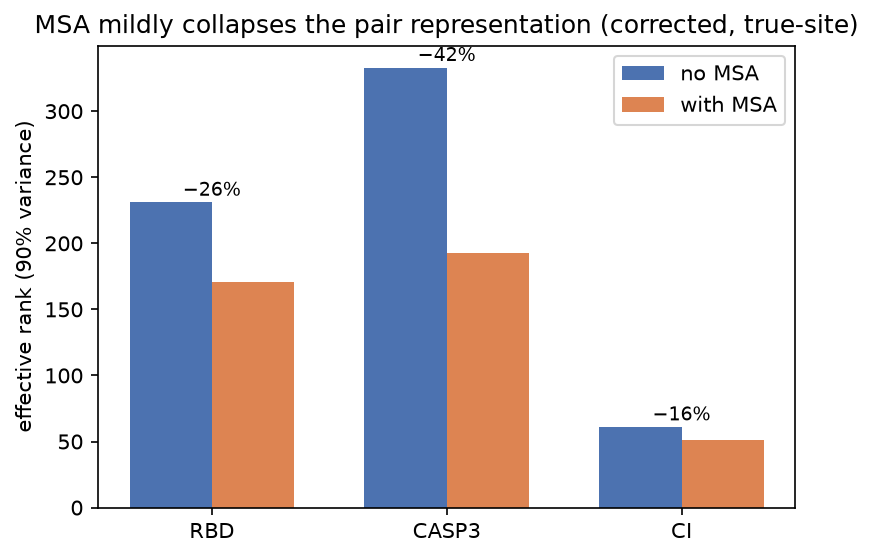
\includegraphics[width=0.85\textwidth]{figures/fig1_geometry_collapse.png}
\caption{\textbf{The MSA mildly compresses the pair representation on three
proteins.} Effective rank at 90\% variance of the centered per-mutant
site-feature ensemble, with and without the MSA (corrected true-site slicing,
full mutant sets). Percentages give the relative rank reduction.}
\label{fig:geometry}
\end{figure}

\begin{figure}[p]
\centering
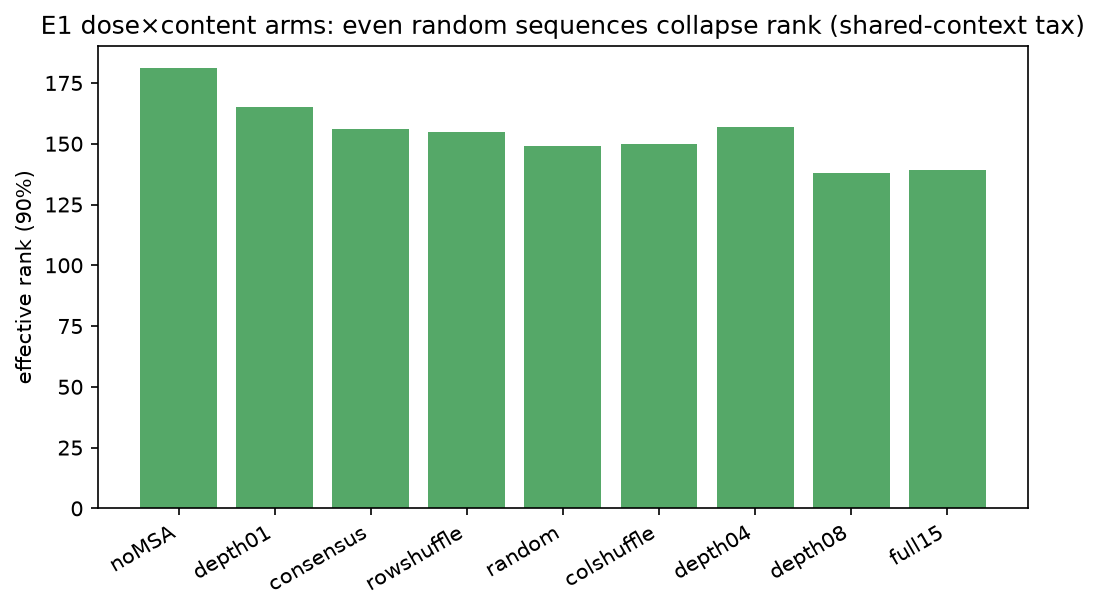
\includegraphics[width=0.9\textwidth]{figures/fig2_arms_effrank.png}
\caption{\textbf{Effective rank across the E1 dose$\times$content arms (RBD).}
Any alignment-like input---including random sequences---compresses the
representation relative to no-MSA (the shared-context tax); the functional
gain, by contrast, requires biological content (Table~\ref{tab:e1}).}
\label{fig:arms}
\end{figure}

\begin{figure}[p]
\centering
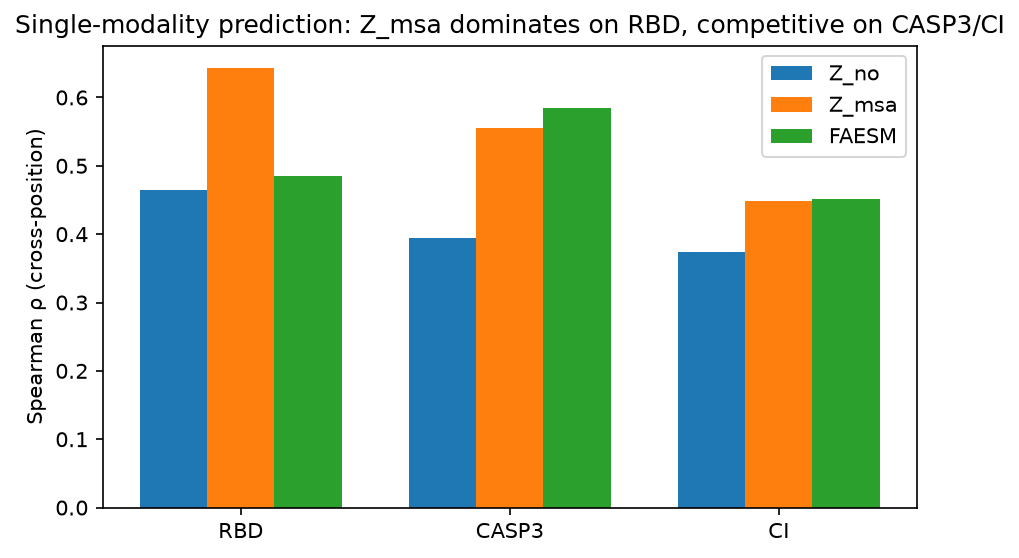
\includegraphics[width=0.85\textwidth]{figures/fig3_single_modality.png}
\caption{\textbf{Single-modality cross-position prediction on three proteins.}
Best-validation Spearman $\rho$ of probes on the no-MSA pair representation
(\Zno{}), the with-MSA pair representation (\Zmsa{}), and ESM-2 embeddings
(FAESM). Values follow the optimistic best-validation convention; de-biased
estimates are given in \S\ref{sec:honest}.}
\label{fig:singlemod}
\end{figure}

\begin{figure}[p]
\centering
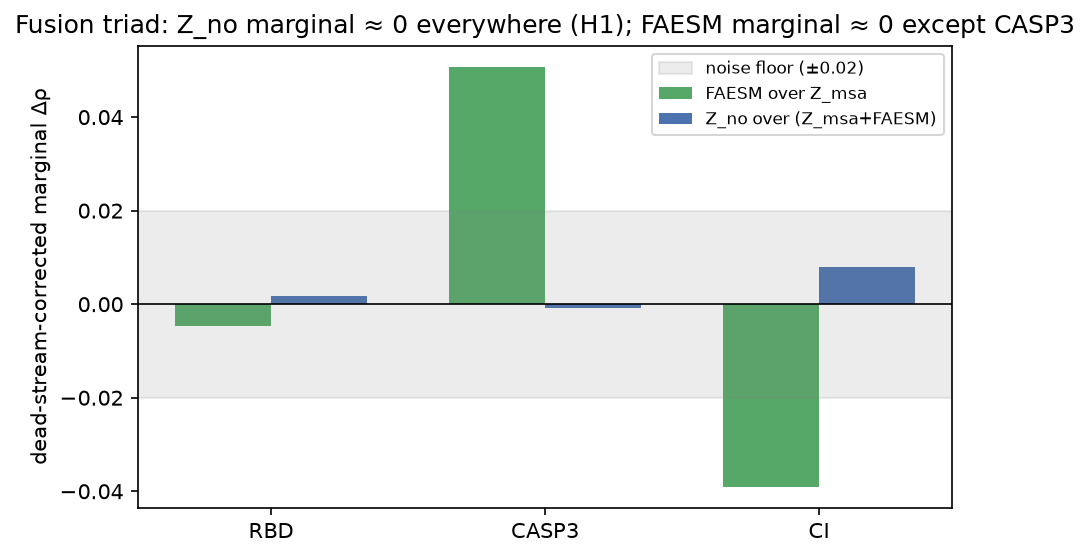
\includegraphics[width=0.9\textwidth]{figures/fig4_triad.png}
\caption{\textbf{Dead-stream-corrected marginals of the fusion triad.} The
no-MSA stream's marginal over $(\Zmsa{+}\mathrm{FAESM})$ is $\approx0$ on all
three proteins; FAESM's marginal over \Zmsa{} is $\approx0$ on RBD, positive
on CASP3, and unresolved (outlier-split-driven) on CI. The shaded band is the
$\pm0.02$ noise floor.}
\label{fig:triad}
\end{figure}

\begin{figure}[p]
\centering
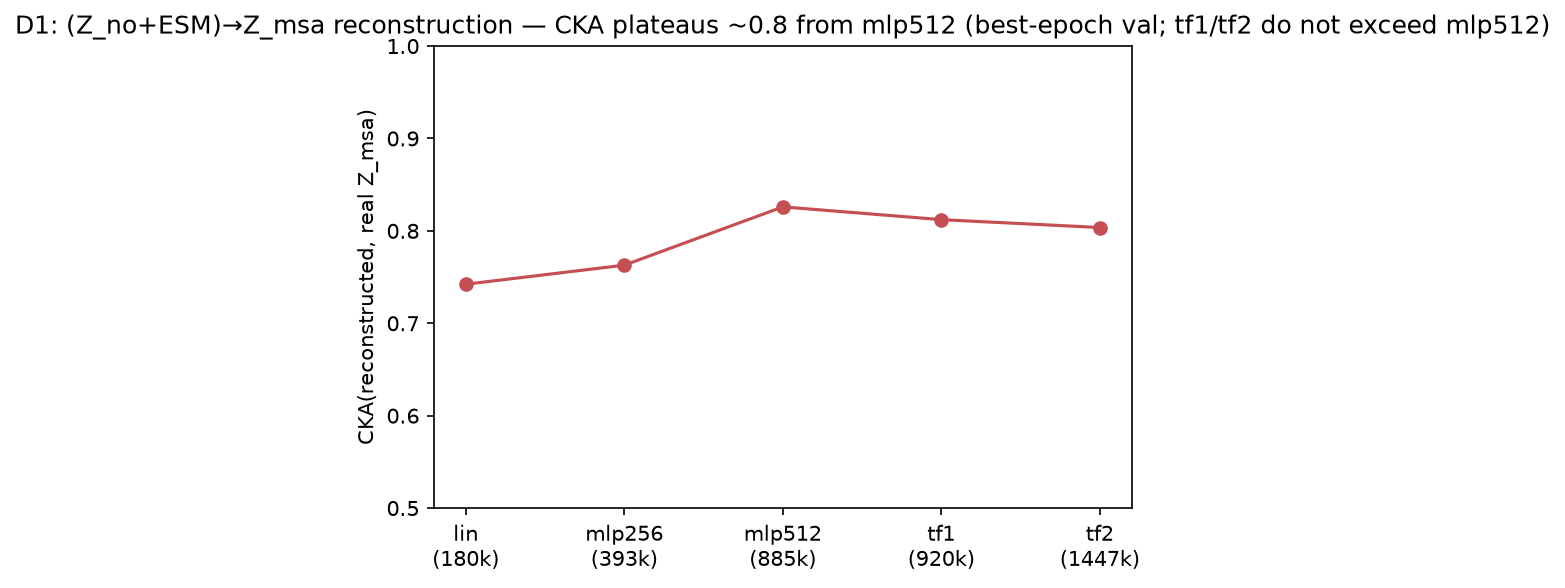
\includegraphics[width=0.9\textwidth]{figures/fig5_d1_capacity.png}
\caption{\textbf{Reconstruction of \Zmsa{} from $(\Zno{},\mathrm{FAESM})$ across
an architecture ladder.} Validation CKA plateaus at $\sim$0.80--0.83 from
MLP-512 (transformers do not exceed it under best-epoch selection);
parentheses give parameter counts.}
\label{fig:d1}
\end{figure}

\begin{figure}[p]
\centering
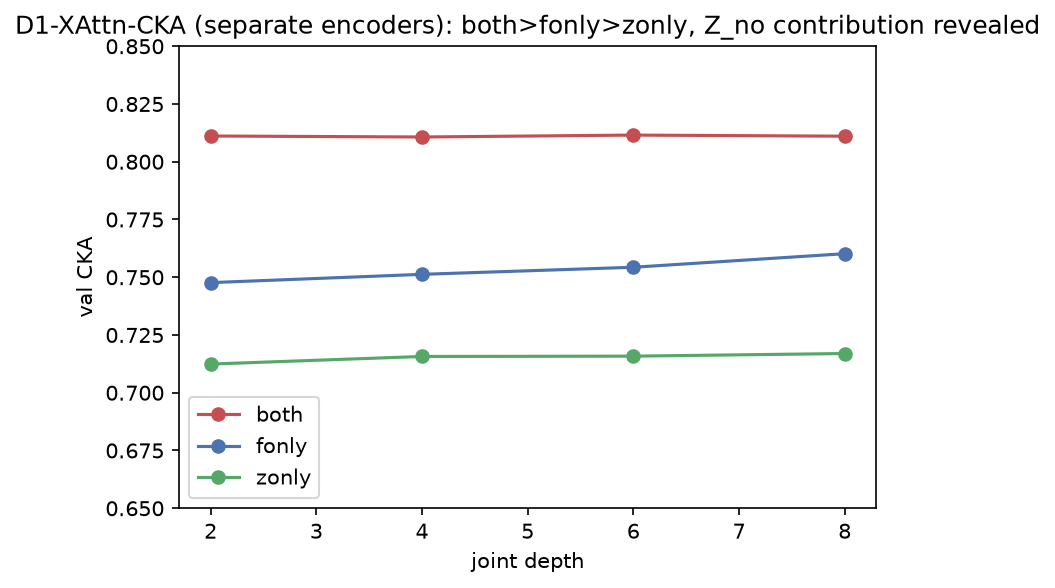
\includegraphics[width=0.9\textwidth]{figures/fig9_xattn_cka.png}
\caption{\textbf{Separate-encoder distillation with a CKA objective.} With
per-modality encoders, the hierarchy is stable across depth: both streams
$>$ ESM-only $>$ \Zno{}-only, showing that the no-MSA pair representation
carries a real contribution that naive concatenation masks.}
\label{fig:xattn}
\end{figure}

\end{document}
